\documentclass[a4paper, 12pt, oneside, polutonikogreek, english]{article}
\usepackage{lmodern}
\usepackage[T1]{fontenc}
\usepackage{csquotes}
\usepackage{booktabs}
\usepackage{url}
\usepackage{textalpha}
\usepackage[dvipsnames]{xcolor}

% Babel package:
\usepackage{babel}
\usepackage{cjhebrew}

\usepackage{eso-pic,graphicx}
\usepackage[top=40mm, bottom=45mm, outer=18mm, inner=18mm]{geometry}
\setlength{\columnsep}{90pt}
%\definecolor{customColor}{RGB}{253, 227, 54}

% With XeTeX$\$LuaTeX, load fontspec after babel to use Unicode
% fonts for Latin script and LGR for Greek:
\ifdefined\luatexversion \usepackage{fontspec}\fi
\ifdefined\XeTeXrevision \usepackage{fontspec}\fi

% ``Lipsiakos'' italic font `cbleipzig`:
\newcommand*{\lishape}{\fontencoding{LGR}\fontfamily{cmr}%
		       \fontshape{li}\selectfont}
\DeclareTextFontCommand{\textli}{\lishape}
\setlength{\emergencystretch}{15pt}
\usepackage{fancyhdr}
\usepackage{amssymb}
\usepackage{array}
\usepackage{float}
\usepackage{imakeidx}
\usepackage{microtype}
\usepackage{setspace}
\onehalfspacing
\makeatletter % change only the display of \thepage, but not \thepage itself:
\patchcmd{\ps@plain}{\thepage}{\bfseries\color{Tan}{\thepage}}{}{}
\makeatother

\color{Tan}
\begin{document}
\bfseries
\renewcommand\thefootnote{\bfseries{\arabic{footnote}}}
\let\oldfootnote\footnote
    \renewcommand{\footnote}[1]{\oldfootnote{\bfseries#1}}
    
\AddToShipoutPictureBG{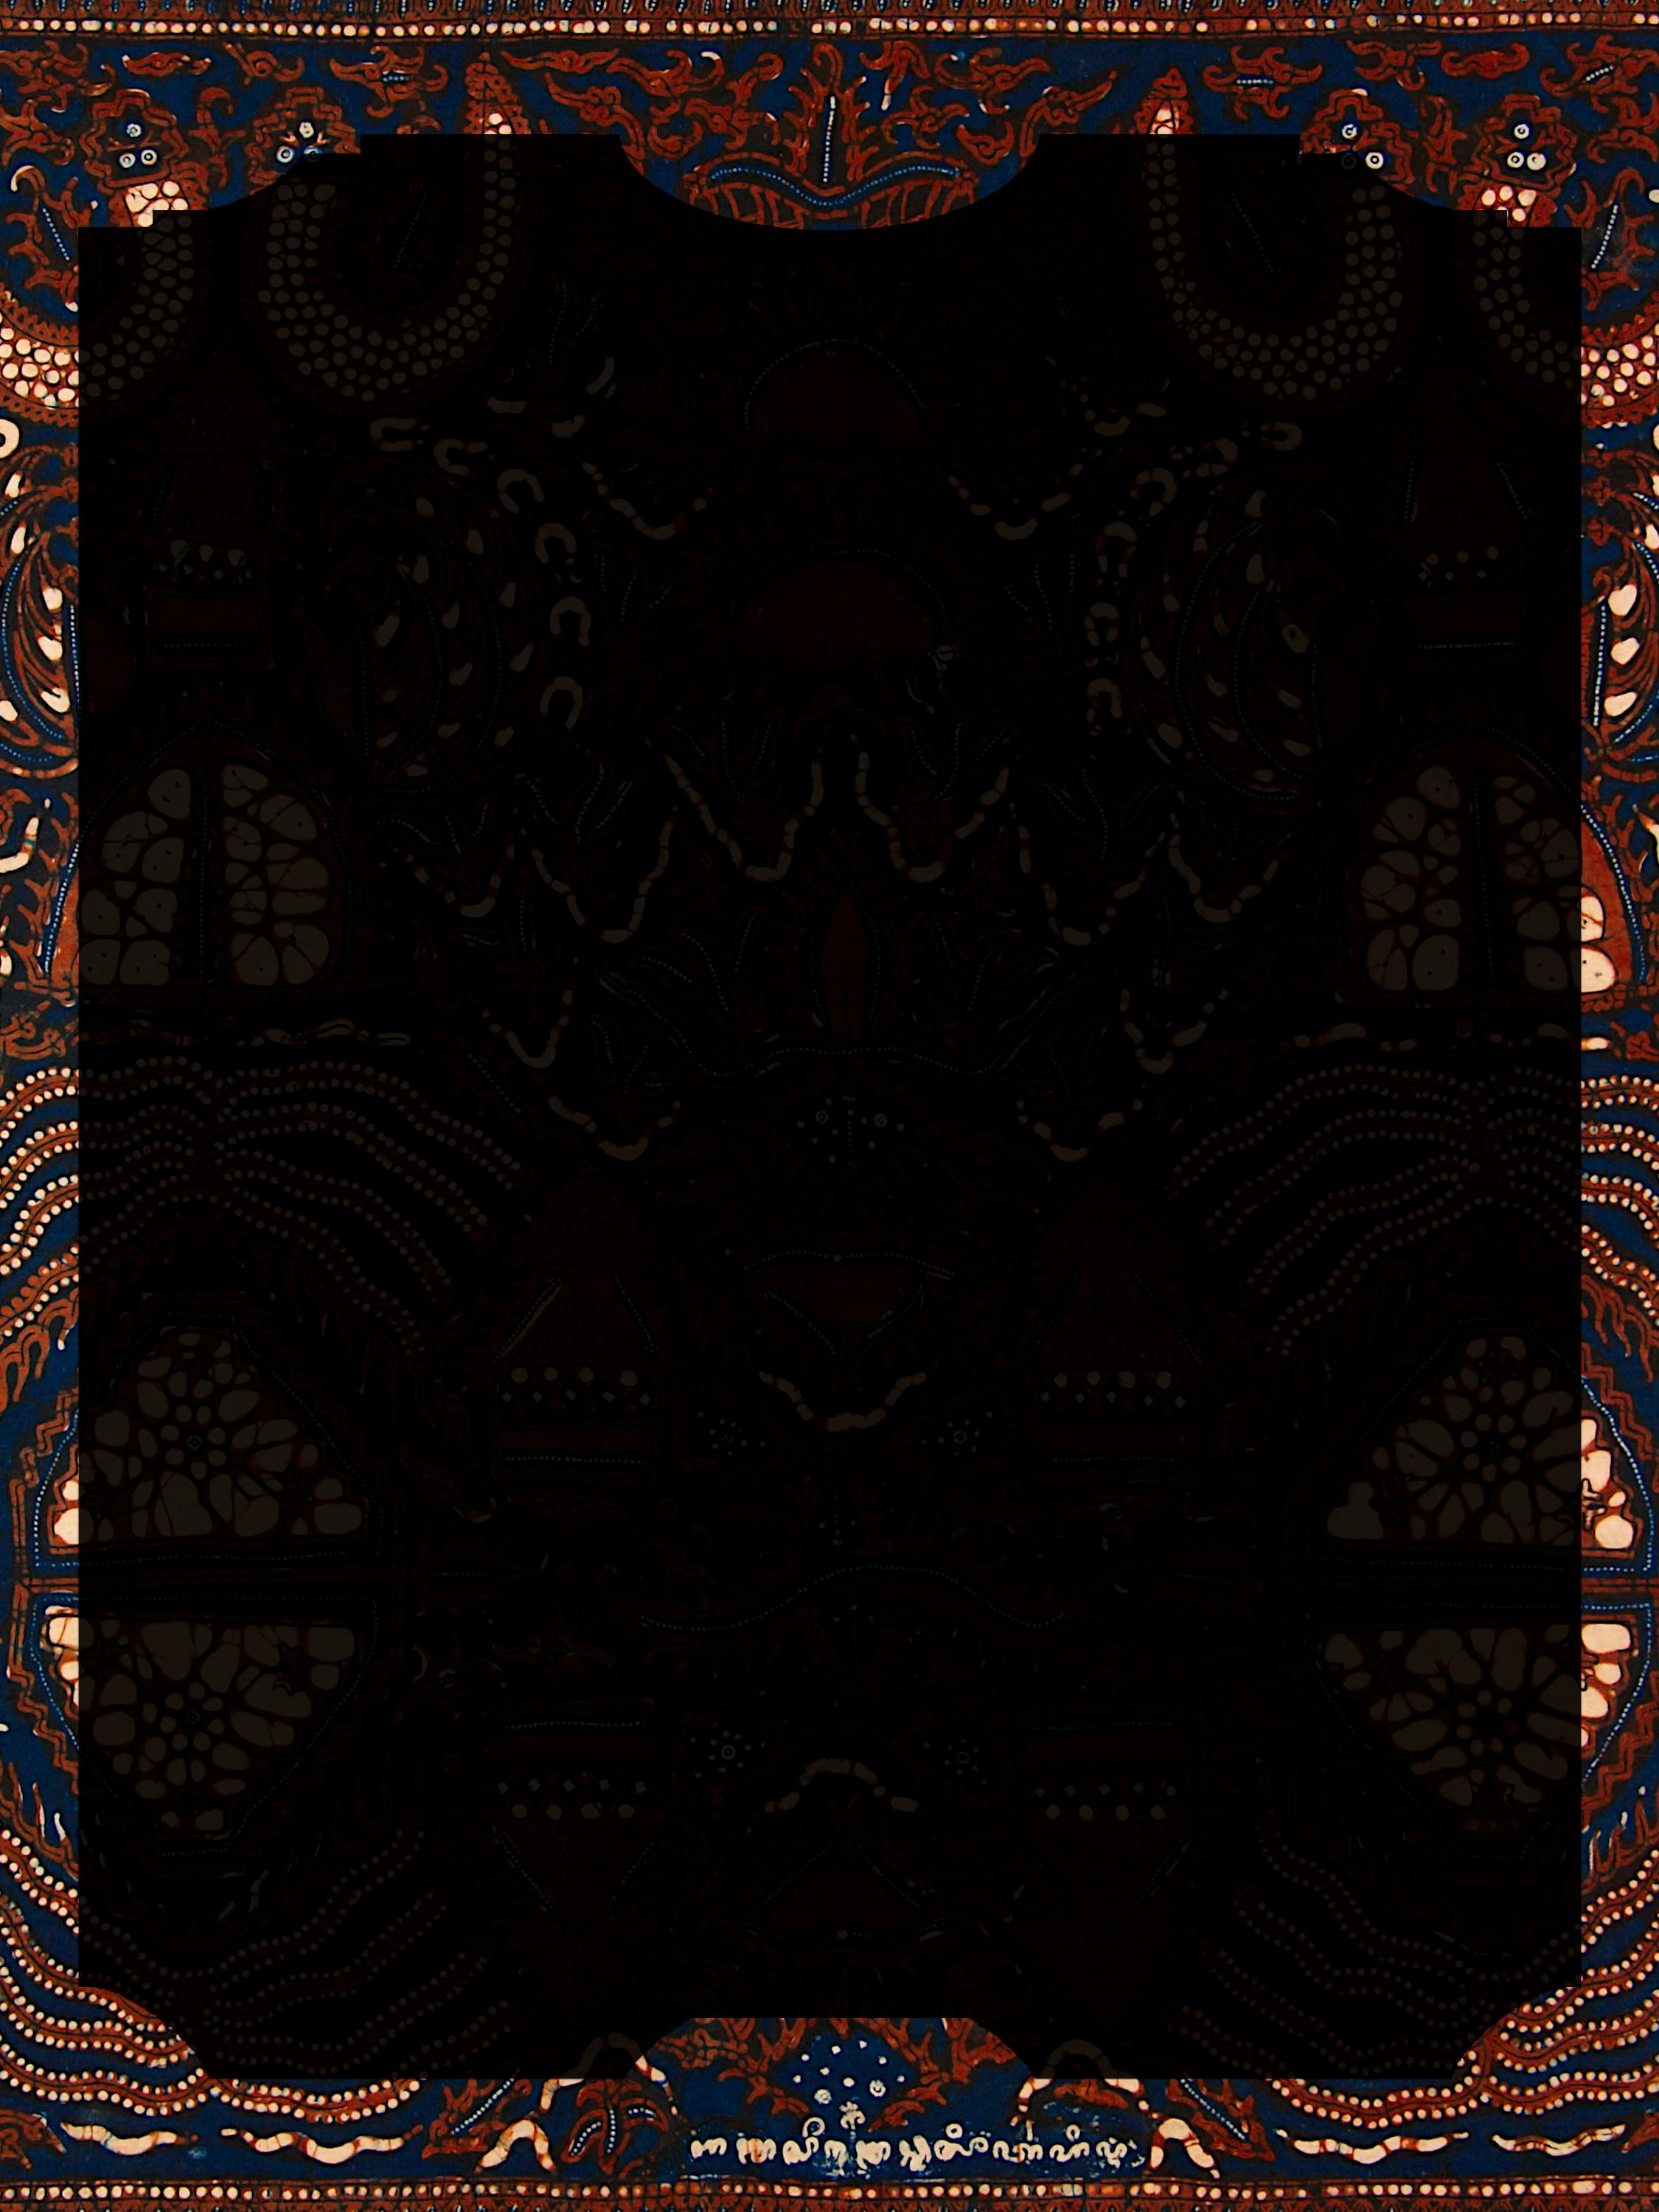
\includegraphics[width=\paperwidth,height=\paperheight]{batik01.jpeg}}
\begin{titlepage} % Suppresses headers and footers on the title page
	\centering % Centre everything on the title page
	\scshape % Use small caps for all text on the title page

	%------------------------------------------------
	%	Title
	%------------------------------------------------
	
	\rule{\textwidth}{1.6pt}\vspace*{-\baselineskip}\vspace*{2pt} % Thick horizontal rule
	\rule{\textwidth}{0.4pt} % Thin horizontal rule
	
	\vspace{0.75\baselineskip} % Whitespace above the title

        {\Huge Baetylia} % Title
	
	\vspace{0.75\baselineskip} % Whitespace below the title
	
	\rule{\textwidth}{0.4pt}\vspace*{-\baselineskip}\vspace{3.2pt} % Thin horizontal rule
	\rule{\textwidth}{1.6pt} % Thick horizontal rule
	
	\vspace{1\baselineskip} % Whitespace after the title block
	
	%------------------------------------------------
	%	Subtitle
	%------------------------------------------------
	
	{By \large George Foot Moore} % Subtitle or further description
	
	\vspace*{1\baselineskip} % Whitespace under the subtitle
	
	%------------------------------------------------
	%	Editor(s)
	%------------------------------------------------
	
	\vspace{1\baselineskip} % Whitespace before the editors

        %------------------------------------------------
	%	Cover photo
	%------------------------------------------------
	
	%\includegraphics[scale=1]{cover}
	
	%------------------------------------------------
	%	Publisher
	%------------------------------------------------
		
	\vspace*{\fill}% Whitespace under the publisher logo
	
	{\small April, 1903}% Publication year
	
	{\small American Journal of Archaeology, Vol. 7} % Publisher

	\vspace{1\baselineskip} % Whitespace under the publisher logo

    Internet Archive Online Edition  % Publication year
	
	{\small Attribution NonCommercial ShareAlike 4.0 International } % Publisher
\end{titlepage}
\clearpage
\large
\paragraph{}
``The worship of holy stones,'' I have written elsewhere, ``is one of the oldest forms of religion of which we have evidence, and one of the most universal. It has frequently persisted in venerable cults in the midst of high stages of civilization and in the presence of elevated religious conceptions, while its survivals in popular superstitions have proved nearly ineradicable.''\footnote{\emph{Encyclopaedia Biblica}, 3, 2279; cf. 3352 f.}

The holy stone was sometimes a natural rock, of striking form or position, \emph{in situ}; sometimes a prehistoric megalith; more frequently a rude block set up for the purpose. It was most commonly of oblong shape, roughly circular or rectangular in section, rounded or pointed at the top. The tapering rectangular block was often fashioned to an obelisk or a pyramid; the round one, to a cone (\emph{meta}) or omphalos. In some places the steps of the further development to rudely iconic forms, and finally to the statue as a work of art, can be traced. On the other hand, the holy stone may grow into an altar on which offerings are made.

Of the origin of this wide-spread phenomenon we may say, as Tacitus does of the sacred stone of Aphrodite at Paphos (\emph{Hist.} 2, 3), ``ratio in obscuro''; but the oldest conception to which we have historical testimony, and the most general in modern times, is that the stone is the seat (ἕδος) of a numen; it is the primitive equivalent at once of temple, idol, and altar.

A distinct class of holy stones are the so-called βαίτυλοι, or βαιτύλια. The earliest mention of these is in the Phoenician History of Philo of Byblos (died under Hadrian), professedly based upon the native work of Sanchoniathon. In \emph{frg.} 2, 19 (\emph{F. H. G.} 3, 568, A), we read, ἐπενόησε θεὸς Οὐρανὸς βαιτύλια, λίθους ἐμψύχους μηχανησάμενος (``Uranos invented baetylia, contriving animated stones''); in the theogony (\emph{ibid.} \emph{frg.} 2, 14; \emph{F. H. G.} 3, 567, B), Uranos and Gē have four sons, --- Ἦλον τὸν καὶ Κρόνον, καὶ Βαίτυλον, καὶ Δαγὼν ὅς ἐστι Σίτων, καὶ Ἄτλαντα.

The baetylia, then, were λίθοι ἔμψυχοι. The modern reader is not unlikely to interpret the words, in the light of animistic theory, ``stones with souls,'' an expression that might apply to any holy stone inhabited by a numen. But Philo --- though, for his time, up in the latest theories of the origin of religion --- had not had the advantage of reading Tylor, and doubtless used ἔμψυχος in the sense in which Plato, \emph{e. g.}, defines it in the \emph{Phaedrus} (245 E),\footnote{See also Arist. \emph{De anima}, 1, 2 (403, \emph{b} 25); \emph{Phys.} 9, 4 (255, \emph{a} 7), self-motion is ζωτικὸν... καὶ τῶν ἐμψύχων ἴδιον. The definition is said to go back to Thales, who attributed life to the lodestone because it moves iron; see Arist. \emph{De anima}, 1, 2 (405, \emph{a} 19) ; Plut. \emph{De placit. philos.} 4, 2, 1; Diogen. Laert. 1, § 24.} πᾶν γὰρ σῶμα ᾧ μὲν ἔξωθεν τὸ κινεῖσθαι ἄψυχον • ᾧ δὲ ἔνδοθεν αὐτὸ ἐξ αὐτοῦ ἔμψυχον • ὡς ταύτης οὔσης φύσεως ψυχῆς, which Cicero (\emph{Tusc.} 1, 23, 54) translates: ``Inanimum est enim omne quod pulsu agitatur externo; quod autem animatum est, id motu cietur interiore et suo; nam haec est propria natura animi et vis.''

The distinctive peculiarity of λίθοι ἔμψυχοι, therefore, is that they are endowed with the power of self-motion. So the words were correctly interpreted by Joseph Scaliger: ``...Baetylos illos fuisse ἐμψύχους et sponte moveri solitos dicunt.''\footnote{\emph{Animadv. Euseb. ad ann.} 2150.}

The appearance and behavior of such an ``animated stone'' is described at length in the Orphic \emph{Lithica}:\footnote{Ed. Abel, v. 360 ff.} Apollo gave Helenus a speaking stone, an unerring lodestone,\footnote{On the marvels of the magnet, see Plin. \emph{N. H.} 36, 126.} which others call ``animated (ἔμψυχον) mountain-stone.'' It was round, roughish, firm, dark colored, dense; its whole surface was covered, in every direction, with wrinkly veins. To obtain a response, the possessor, after a period of purification, bathed the knowing stone, swaddled it like a babe, and, by sacrifices and incantations, got it to breathe; then, after he had dandled it a long time, it suddenly started up the cry of a new-born infant --- woe to him if, in alarm, he let it fall! To any question now put to it, it returned an infallible response; then, if closely watched, it would be seen miraculously to cease breathing (θεσπεσίως... ἀποψύχοντα).

Damascius,\footnote{Preserved in Photius, \emph{Bibliotheca Codicum}, cod. 242, p. 348 Bekker = Migne, \emph{Patrol. Graeca}, 103, 1292 f.} in his life of Isidorus, gives us similar descriptions of the baetylia, which were particularly common in the region of the Lebanon. A certain Eusebius, who was the possessor --- or, rather, minister (θεραπεύων) --- of a baetyl, told the story that one night he had a sudden impulse to wander, from the city of Emesa, to a mountain a long way off, on which was an ancient temple of Pallas. While he was resting himself there, he saw a ball of fire rushing down from on high; when it reached the earth there appeared beside it a lion, which presently vanished. When Eusebius approached the spot, he found the stone cooled off, and, recognizing that it was a baetyl, took it home with him. Damascius describes it as an exact sphere about nine inches in diameter, of a dull white color, though it varied in size, and sometimes turned purplish. There were letters on the stone, colored with vermilion, through which responses were given to inquirers. The stone also emitted a thin, piping voice, which Eusebius interpreted.

Eusebius's baetyl belonged to a god, Gennaios, who was worshipped at Heliopolis in the form of a lion; others were dedicated to other deities, such as Kronos, Zeus, or Helios.

Damascius thought the baetyl was something divine, but Isidorus held that it was a daemon that moved it --- one of the kind that is neither very bad nor very good.

In another place\footnote{Photius, \emph{op. cit.} 342 Bekker = 1273 Migne.} Damascius says that, in the vicinity of the Syrian Heliopolis, Asclepiades went up on Mt. Lebanon and saw many of the so-called baetylia, ``about which he tells many marvels.'' Damascius himself had seen a baetyl moving through the air, and again hidden from sight in its garments or carried in the hands of its minister.

From Damascius is derived the wisdom we find in the \emph{Etymologicum Magnum}, and in Zonaras, Βαίτυλος, λίθος γενόμενος κατὰ τὸν Λίβανον τὸ ὄρος τῆς Ἡλιουπόλεως.

A Christian writer of uncertain date, Joseph, the author of the \emph{Hypomnesticon},\footnote{First printed in Fabricius, \emph{Codex Pseudepigraphus V. T.} 2, 326 ff., then by Galland, \emph{Bibl. Vet. Patr.} 14, 3 ff., Migne, \emph{Patrol. Graeca}, 106, 16 ff.} in a chapter on various forms of pagan divination, writes: χρηστήρια διαβόητα παρ᾽ αὐτοῖς ἐστι τὰ ἐν τοῖς ναοῖς βαιτύλια διὰ λίθων ἐν τοῖς στοιχείοις προσρασσάντων.\footnote{A footnote (? gloss) in Fabricius adds, βαιτύλια λίθοι ἔμψυχοι ἐν ἀέρι κινούμενοι.}

Sotacus of Carystus (Plin. \emph{N. H.} 37, 135) classed the baetylia with the \emph{cerauniae gemmae}, of which there are two kinds, black and red, resembling axes; the black, round ones are sacred; by means of them cities and fleets are captured, --- these are called baetyli, --- while the long ones are ``ceraunian'' in the narrower sense.

The word βαίτυλος; occurs in only one other connection. In the lexica it is explained as the name of the stone which was given to Kronos to swallow in place of the infant Zeus. Thus the \emph{Etymol. Magn.}, \emph{s. v.}: Βαίτυλος δὲ ἐκλήθη καὶ ὁ λίθος ὃν ἀντὶ Διὸς ὁ Κρόνος κατέπιεν • εἴρηται δὲ ὅτι ἡ Ῥέα βαίτῃ αἰγὸς σπαργανώσασα τῷ Κρόνῳ δέδωκε • βαίτη δὲ σημαίνει τὴν διφθέραν.

This statement is found in substance in several other lexicographers and grammarians: Herodian, Περὶ καθολικῆς προσῳδίας, 6 (ed. Lentz, 1, 163); Hesychius (ed. M. Schmidt, 1, 353); Theognostus, Κανόνες, 61, 21 (Cramer, \emph{Anecdota Oxon.} 2); Λέξεις Ῥητορικαί (Bekker, \emph{Anecdota Graeca}, 1, 224); \emph{Etymol. Gudianum}, \emph{etc.} Here belongs, also, the proverb from Arsenius's collection (Leutsch, \emph{Corpus Paroem.} 2, 468): καὶ βαίτυλον ἂν κατέπιες • ἐπὶ τῶν ἄγαν λιμβῶν. βαίτυλος δέ ἐστιν ὁ ἐσπαργανωμένος λίθος ὃν Kρόνος κατέπιεν ἀντὶ τοῦ Διός. A comparison of these passages plainly shows that they are all ultimately derived from one source.

The myth of Kronos devouring his offspring and the fraud by which Zeus was saved from this fate\footnote{Hesiod, \emph{Theog.} 468 ff. Represented on an altar relief in Rome (Overbeck, \emph{Kunstmythologie}, 2, 326 ; Baumeister, \emph{Denkmäler}, 2, 798) and on a red-figured vase of Sicilian origin (J. De Witte, \emph{Gazette Archéologique}, 1, 30 ff. and pl. 9). According to Paus. 9, 2, 7, the scene was represented in a temple of Hera at Plataea.} is Cretan; the god of whom it is told is evidently related to the Phoenician Kronos (El), of whom Philo of Byblos relates that he killed a son and daughter with his own hands (\emph{frg.} 2, 18; \emph{F. H. G.} 3, 568), and on more than one occasion sacrificed his own children (\emph{ibid.} \emph{frg.} 2, 24; 4 f.).

The Semitic word\footnote{See below, p. 203.} βαίτυλος itself, of which the Greeks give far-fetched etymologies, connects the Cretan myth with the Phoenicians. The presumption, therefore, is that the stone which was shown in Crete as the Zeus stone was really such a baetyl as those in the Lebanon described by Damascius. Direct evidence of this is lacking; but two passages may at least be cited in this connection: Porphyry, in his life of Pythagoras (§ 17), narrates how Pythagoras in Crete visited the mystae of Morgos, one of the Idaean Dactyls,\footnote{The Idaean cave as place of Zeus's birth, in later poets, \emph{etc.}; see Callim. \emph{In Jov.} 4 ff.; Preller-Robert, 1, 133.} and by them was purified ``with the ceraunian stone,'' after which he went down into the Idaean cave, \emph{etc.} The other passage is a note of Tzetzes on Lycophron, l. 400: Δίσκον δὲ τὸν Δία λέγει διὰ τὸν λίθον τὸν ἀντὶ Διὸς ὑπὸ Ῥέας σπαργανωθέντα καὶ ὑπὸ Κρόνου καταποθέντα, ὥς φησιν Ἡσίοδος ἐν τῇ Θεογονίᾳ κ. τ. λ.

We read in Hesiod (\emph{Theog.} 497-500) that, when Kronos had disgorged the stone, Zeus set it up at Delphi, ``to be a sign in after times and a marvel to mortals.''\footnote{A. Meyer (1887) and Peppmüller (1896) reject vv. 492-500, as well as 501-506, which are more generally regarded as an interpolation.} Pausanias (10, 24, 6) was shown there a stone, of moderate size, on which oil was daily poured, while on every feast day white wool was placed upon it; it was reputed to be the stone that was given to Kronos instead of his son.

There is no reason to believe that the stone at Delphi had actually been transported thither from Crete, as the stone of the Mater Deum of Pessinus or that of Elagabalus of Emesa was brought to Rome. The probability is vastly greater that the foreign myth was simply attached to an old Zeus stone at Delphi,\footnote{Schoemann, \emph{De incunabulis Jovis}, 7 f. = \emph{Opusc. Acad.} 2, 254, who, however, erroneously thinks that the myth started at Delphi.} just as the scene of the deception of Kronos was localized at Chaeronea (Paus. 9, 41, 6). In later times the Terminus on the Capitol at Rome was identified with the stone which Saturn had swallowed (Lactant. 1, 20, 37). Perhaps the local custom of covering the holy stone at Delphi with wool suggested the λίθος ἐσπαργανωμένος of the myth.

However that may be, there is neither in the tradition nor in the facts as reported to us any warrant for applying the name βαίτυλος to the Delphian stone, as modern writers often do.

The word βαίτυλος is of Semitic origin --- more specifically, as the vowels show, Phoenician. \emph{Bait-yl}, corresponding to Hebrew \emph{bēth-ēl}, may be translated \emph{ad verbum}, ``house of god''; but, as often, the seeming exactness of the literal rendering is misleading. \emph{Ēl} (Phoen. \emph{Yl}) is a much vaguer word than our ``god'' --- it is merely δαιμόνιον; we may approximately render it ``supernatural power''; and \emph{bait} in such compounds is a place where, or a thing in which, something is. \emph{Bait-yl} therefore is, more properly, ``a thing in which is a supernatural power, a daemonic life.'' It admits equally the opinion of Damascius, who thought θειότερον εἶναι τὸ χρῆμα τοῦ βαιτύλου, and that of Isidore, εἶναι... τινα δαίμονα τὸν κινοῦντα αὐτόν.\footnote{See above, p. 200.}

A synonym of \emph{baetylus} is \emph{abaddir}. Priscian (7, 32, ed. Hertz, 1, 313) writes: ``\emph{Abaddir} βαίτυλος... lapis quem pro Iove devoravit Saturnus.'' That this also was a λίθος ἔμψυχος appears from Mythogr. Vatican. (\emph{Scriptores Rerum Mythicarum Lat.} ed. Bode, p. 34): Rhea ``misit Saturno gemmam in similitudinem pueri celsam, quam abidir vocant, cuius natura semper movetur.''

Augustine (\emph{Ep.} 17, 2, \emph{ad Maxim.}), replying to the pagans, says: ``miror, quod nominibus absurditate commoto in mentem non venerit habere vos et in sacerdotibus Eucaddires et in numinibus Abaddires.'' An inscription from Mauretania (\emph{Ephem. Epigraph.} 7 no. 529) reads: ``abaddiri • sa|ncto • culto|res • iuniores suis sumpt | aram constitu | pro...'' The word occurs frequently in Latin glossographers, --- who need not be quoted here, --- as equivalent to baetylus, with or without the story of Saturn and Rhea.

The word \emph{abaddir}, like \emph{baetylus}, is of Semitic origin; Augustine's reference is to its use by the Punic population of North Africa; from Mauretania comes the inscription of the \emph{cultores juniores}. The natural interpretation of the name is ``mighty or noble father''; the epithet \emph{addir} is repeatedly applied in the Old Testament to God, and occurs in other Phoenician compound names; cf. \emph{Baliddir} in a Numidian inscription (\emph{Ephem. Epigraph.} 7, no. 792).

Upon the question what the baetylia really were, I do not propose to enter here. They were believed to be fallen from heaven, that is, to be small aerolites, and in some instances they may have been such; but, in the light of kindred beliefs in many parts of the world, it is probable that they were generally prehistoric stone implements, especially axes and ``mace heads.''\footnote{Cf. Plin. \emph{N. H.} 37, 135, ``similis eas esse securibus.'' They were not belemnites, of which Pliny speaks, as a third class, in the following sentence. On stone axes regarded as thunderbolts, see Lenormant, \emph{Revue de l'Hist. des Religions}, 3, 48, Daremberg et Saglio, \emph{s. v.} Bétyles, with references; further, J. Evans, \emph{Ancient Stone Monuments}, 62 ff.; A. J. Evans, \emph{Journ. Hellen. Studies}, 21, 118. Greek peasants still call stone axes ἀστροπελέκια (Dumont, \emph{Rev. Archéol.} N. S. 15, 358). The same belief about white jade axes in China (Keane, \emph{Man Past and Present}, 219); among the Shans (\emph{ibid.} 172); in Mexico (Ratzel, \emph{History of Mankind}, 2, 152), \emph{etc.}}

It appears, from the examination of all the evidence, that the name βαίτυλοι was appropriated to certain small stones of peculiar character, to which various daemonic --- or, as we might say, magical --- properties were ascribed; they moved about, talked, or otherwise answered questions, and afforded a powerful protection to their possessors. There is no evidence that the name was anywhere applied to the ordinary holy stones, --- cones, pillars, omphaloi, or the like.\footnote{See Falconnet, \emph{Mem. Acad. Inscr.} 6, 523 (1722), where the whole matter is correctly stated.}

Many modern writers, on the contrary, employ the term of the latter specifically. Thus, L. Schmitz, in Smith's \emph{Dictionary of Biography and Mythology}, \emph{s. v.}, writes: ``Baetylus (βαίτυλος) is in reality the name of a peculiar kind of conical-shaped stones, which were erected as symbols of gods, in remarkable places, and were, from time to time, anointed with oil, wine, or blood.'' And --- not to name any others --- Sir Arthur Evans, in his instructive `Mycenaean Tree and Pillar Cult,'\footnote{\emph{Journ. Hellen. Studies} (1901), 21, 99 ff., and separately.} constantly uses the word \emph{baetylos} in the sense of ``stone pillar,'' ``the aniconic image of the divinity'' (p. 113); he applies the name ``baetylic altars'' to a type of altar or table supported by four legs over a central, slightly tapering stone, and thinks that in one of these the stone may, perhaps, represent the actual Cretan \emph{baetylos} of Zeus (§ 6); he even speaks of sepulchral stelae as ``baetylic habitations of departed spirits'' --- so completely has the word become for him a name for any \emph{cippus} conceived to be the seat of a numen or spirit.\footnote{The presentation of the subject is not free from minor errors of fact, as when (p. 113) the author says that the name βαίτυλος was ``applied to the black cone representing the Sun God at Baalbec.'' The \emph{Etymol. Magn.}, which is cited in support of this statement, says nothing of the kind.}

The origin of this deflection of the word to a use so contrary to that which it has in the ancient authors is an interesting and instructive chapter in the history of learning. In the sixteenth and seventeenth centuries the theory prevailed that heathen rites and customs were, in great part, perversions of the purer primitive religion whose record we have in the Old Testament.\footnote{The theory is, of course, much older.} The anointing of holy stones (λίθοι λιπαροί) was thus a perversion to idolatry of a patriarchal precedent.\footnote{Falconnet cites as adherents of this opinion, besides Bochart and Scaliger, G. J. Voss, Grotius, Selden, Huet, Heidegger, Witsius, \emph{etc.}} In his flight to Syria, Jacob passed a night at a place called Luz. Having taken one of the stones of the spot as a pillow, he slept, and in his dream saw a ladder reaching from the earth to heaven and the messengers of God ascending and descending upon it. The vision showed him that the place was an abode of divine beings, the entrance of heaven. In the morning he took the stone that was under his head, set it up as a pillar (\emph{maṣṣēbāh}), poured oil upon it, and vowed that, if he returned in safety, this stone should become a temple (\<byt 'lhym>); this was the way that the place came to be called Bethel (\<byt'l>).\footnote{Gen. 28.}

The name \emph{bēth-ēl} naturally suggested the βαίτυλοι. Joseph Scaliger, after referring to the anointing of holy stones, and to the βαίτυλοι of Philo of Byblos and the βαίτυλος which Saturn swallowed, wrote: ``omnemque hunc morem manasse ab eo lapide, quem unxerat Jacob in Bethel.''\footnote{\emph{Animadv. Euseb. ad ann.} 2150.}

One of the most learned --- and most perilously ingenious --- of French scholars, Bochart, went a step farther. He not only explicitly derives the name \emph{baetylia}, \emph{baetylus}, from the place Bethel, but, by a bold emendation in ``Sanchoniathon,'' the alleged Phoenician original of Philo, he identifies the objects with \emph{lapides uncti}. Philo, as we have seen, calls the baetylia λίθοι ἔμψυχοι. ``Live stones,'' says Bochart, ``is a contradiction in terms, an absurdity; instead of \emph{nĕphāshīm} (`animati'), Sanchoniathon doubtless wrote \emph{nĕshāphīm} (`uncti'),\footnote{Perhaps it is not superfluous to say that this ``Phoenician'' is purely fictitious.} from the root \emph{shūph}, used in Syriac in the sense `anoint.''' Then, after quoting the story of Jacob, he continues: ``The Phoenicians, with an unhappy imitation of this example, first worshipped the stone which the patriarch had set up; then they anointed and consecrated other stones, and called them baetylia, baetyli, in memory of the stone at Bethel.''

To the conclusive refutation of Bochart by Falconnet no attention was paid, while the whole long passage from the \emph{Geogr. Sacra}, in which Bochart set forth his theory, has been incorporated bodily in modern editions of the Greek \emph{Thesaurus}, through which its philological and historical errors have filtered into the encyclopaedias and hand-books of classical archaeology.\footnote{Tümpel, \emph{e. g.}, in Pauly-Wissowa, \emph{s. v.} \emph{abaddir}, reproduces Bochart's impossible etymology.}

Classical scholars the more readily accepted this erroneous theory, because they incautiously assumed that the name βαίτυλος, given in the lexicographical tradition to the stone swallowed by Kronos, referred --- or might be referred --- to the stone at Delphi, of which the same story was told. Since this was daily anointed with oil, the connection with the stone pillar which Jacob anointed at Bethel seemed to be doubly secured.

Many modern Old Testament students, on their side, surmise that the name \emph{bēth-ēl} originally belonged, not to the place, but to the holy stone itself as ``the abode of a divinity,'' corresponding thus, in fact as well as in name, with the ``fetish-stones'' which the Greeks designated by the foreign word βαίτυλοι.\footnote{See, \emph{e. g.}, Gunkel, \emph{Genesis}, 290.}

It must be borne in mind, however, that this theory is suggested, not by anything in the Hebrew accounts in Genesis, but solely by the etymological association with the βαίτυλοι and by the ``baetylic'' theories of classical scholars. What is much more important to observe is that in no Semitic language is the word \emph{bēth-ēl} or its equivalent used to designate the rude standing stones, pillars, obelisks, and the like which were found at every place of worship. The argument from silence is of more than usual force, because the references to these stones are so numerous, and the various names by which they were called so abundantly attested.\footnote{See \emph{Encyclopaedia Biblica}, \emph{s. v.} Massebah.} In Phoenician we know them from inscriptions on the objects themselves.

Summing up, then, the results of this investigation --- which may fairly claim to be exhaustive --- we may say that there is no evidence, either from Semitic sources or from Greek and Latin authors, that the name \emph{baetylus} was ever applied in antiquity to the class of objects which modern archaeologists habitually call ``baetyls''; on the contrary, it was the distinctive designation of an entirely different thing.

It is to be hoped that the abuse of the term may not become unalterably fixed. There is no lack of names properly applicable to the common holy stones; there is no other convenient word for the real \emph{baetylia}.

\bigskip

George F. Moore.
\end{document}
